\documentclass[a4paper,12pt,oneside]{article}
\usepackage{achemso}
%\usepackage{graphicx} 
\usepackage{epsfig}
\usepackage{enumerate}
\usepackage[normalem]{ulem}
\graphicspath{{images/}}
\begin{document}
\title{Interface Builder ver. 0.0.2 - user manual}
\author{Jakub Kami{\'n}ski
\\
Department of Mathematics,
University of California Los Angeles \\
}
\maketitle
\section{Introduction}
This document provides manual for the Interface Builder. The program is still in
development stage as new features are being constantly added. At this stage the
focus is more on the underlying theory and algorithms, whereas end user
experience is put to the background. Once the development part is considered
complete, the complete user interface will be created. 

The program execution is controlled with the external input file.  
The compatibility between all the keywords combination has not been throughly 
tested, and some might lead to error.

The run-time exception handling routines has been added to the program,
particularly in the
most sensitive places: \textit{i)} crystal lattice reduction, \textit{ii)}
finding of the primitive vectors of the given superlattice. In those cases, the
program will stop execution and return with (hopefully meaningful) error
message. 
\section{Functionality} 
The program is intended to construct interfaces from various materials for which
surface orientation specified by Miller indices. In the most general case, user
supplies the program with the range of Miller indices to be considered,
and program explores all the possible combinations. As the result, user gets the
set of all the possible structures (organized in the directories), as well as
the summary file for further analysis.

\section{Installation}
\subsection{Python}
The program is written in Python 2.7. It uses standard Python modules + Numpy. 
In most modern Linux distributions and MacOS Python is pre-installed together
with Numpy package. On Windows machines, Python and Numpy require additional
installation.
\subsection{Program execution}
This manual will cover usage of Interface Builder in Unix based environments. 
\noindent
Before first execution, make sure that the script is executable:
\begin{verbatim}
chmode +x IfaceBuilder.py
\end{verbatim}

\noindent
To execute the program, in the same directory issue:
\begin{verbatim}
./IfaceBuilder.py options.dat
\end{verbatim}
where \texttt{options.dat} is the file with options controling program
execution.

\section{Program options}
The options to the program are supplied in \texttt{options.dat} file.
\textbf{The structure of the \texttt{options.dat} is very rigid, order of
options matter, all the supplied keywords are case sensitise.} Again, there are
no error handling routines avaialble in the code, therefore mistakes
in the
options file will not be detected. More modern
implementation allowing for more freedom will be done later, once the code will
reach end of development cycle.

\subsection{Structure of \texttt{options.dat} file}
The rigid file structure is given as follows:
{\small
\begin{verbatim}
substrate     Si-opt.cif   # CIF file for Substrate
substrateIDX  2            # Miller indices for Substrate
deposit       Al.cif       # CIF file for Deposit
depositIDX    2            # Miller indices for Deposit
maxArea       150          # Maximum area of lattices
areaThresh    5.0          # Threshold for area misfit    [in %]
vecThresh     5.0          # Threshold for vectors misfit [in %]
angleThresh   5.0          # Threshold for angle misfit   [in %]
capAtmSub     None         # Atom to cap the substrate exposed surface or None
capAtmDep     None         # Atom to cap deposit exposed surface or None
fparam        1            # Parameter f for scoring function
nLayerS       18.5         # Thickness of Substrate slab [A]
nLayerD       17           # Thickness of Deposit slab [A]
noConf        2            # Desired number of configurations to return
subAtRad      1.25         # Substrate atomic radius
depAtRad      1.17         # Deposit atomic radius
skipStep1     True         # Skip automatic generation of slabs distance True/False
poissonRatio  True         # Scale z-axis in the Deposit according to Poisson ratio
sandwich      False        # make a sandwich configuration S-D-S
nVac          4            # Amount of vacuum layers above the slab
\end{verbatim}
}
\noindent
We will follow explaining each option one by one.
\begin{itemize}
\item{\texttt{substrate   Si.cif}}\\
Name of the CIF file with substrate structure. \uline{The .cif file needs to be in the same directory as the IfaceBuilder.py}

\item{\texttt{substrateIDX  n}}\\
This option specifies the Miller indices of the \texttt{Substrate} plane. There
are two ways how one can specify Miller indices:
\begin{enumerate}[I.]
\item Specify range of Miller indices by suppling integer number from 1-9,
for instance \texttt{substrateIDX  2}. In that case, InterfaceBuilder will
generate all the possible combinations of Miller indices in the form
\texttt{(hkl)}, where \texttt{h,k,l} take values from \texttt{0,...,n}. For
example, if
\texttt{n=1} then InterfaceBuilder will generate all combinations
(001),(010),(100),(011),(101),(110),(111). Specifying \texttt{n=2} will give all
the combinations (001),(002), (012),(022),...,(222).
\item Specify desired Miller index explicitly in the form \texttt{hkl}, for
instance \texttt{substrateIDX  111}. In this case only one plane for the
\texttt{Substrate} will be created.
\end{enumerate}

\item{\texttt{deposit} and \texttt{depositIDX}}\\
Same as \texttt{substrate} and \texttt{substrateIDX} but for Deposit.

\item{\texttt{maxArea       250}}\\
Maximum allowed interface area. In Angtroms. 

\item{\texttt{areaThresh    5.0}, \texttt{vecThresh     5.0},
\texttt{angleThresh   5.0}} \\
Maximum thresholds for Area, Lattice vectors and Angles between lattice vectors
given in \%. Decreasing those numbers will give fewer candidate structures, but with
better fit. Decreasing those number will give give more candidate structure, but
with bigger misfit. 

\item{\texttt{capAtmSub     Cl}}\\
Capping atom for the exposed surface of Substrate. Capping atoms are placed in
the positions of the atoms that would be there in the true material. This
implementation follows the new method to calculate the polar surface energies
that is still under development, therefore this feature is also not very
universal. \uline{Setting this option to \texttt{None} disables capping atoms.}

\item{\texttt{capAtmDep     H}}\\
Same as \texttt{capAtmSub} but for Deposit.

\item{\texttt{fparam   1}}\\
Parameter \texttt{f} for Scoring function

\item{\texttt{nLayer  18.5}}\\
Thickness of the Deposit and Substrate. In Angstroms. 
Manipulating this value for non-polar materials, one can find exposed 
surfaces that are "better"
terminated than the other ones, i.e. having only one dangling bond instead of two. 

\item{\texttt{noConf   8}}\\
Limits the number of output structures to the given number. 
If the given number is bigger than the actual number of structures, all the 
structures will be printed. 

\item{\texttt{subAtRad   2.20}}\\
Atom radii of the atoms in Substrate. This is needed for the SCORING function. 

\item{\texttt{depAtRad   2.20}}\\
Atom radii of the atoms in Deposit. This is needed for the SCORING function.

\item{\texttt{skipStep1  True}}\\
Setting this option to \texttt{False} will use SCORING function to determine the
optimal distance between the Substrate and Deposit slabs. It increases the time
to output structures considerablt. 
If it is set to \texttt{True}, the array with the desired distances between
Substrate and Deposit slabs needs to be specified. Up to today, this is not
possible to do from the level of the options file, but it requires manual
inspection of \texttt{IfaceBuilder.py} script. This is not as hard as it seems.

To do so, open the \texttt{IfaceBuilder.py} with text editor and go to line no.
\texttt{3798}. The following variable should be defined there:
\begin{verbatim}
if skipStep1:
        bondlist = [0.9,1.6,1.9,1.4,2.0]
\end{verbatim}

\noindent
The numbers in the \texttt{bondlist} array are multipliers of average of atomic
radii $r_{avg}=\frac{r_{Sub}+r_{Dep}}{2}$ ($r_{Sub}$ and $r_{Dep}$ given in
\texttt{subAtRad} and \texttt{depAtRad}). Specifying, for instance, multiplier
to \texttt{0.9} means that the Substrate and Deposit will be placed $0.9r_{avg}$
apart. The length of \texttt{bondlist} depends on number of alignments, that 
are created automatically, and can be found by running code once and noting the
printed number.

\item{\texttt{poissonRatio True}}\\
When creating interface, the \texttt{a} and \texttt{b} lattice vectors of
Deposit are 
always scaled to exactely match the
\texttt{a} and \texttt{b} lattice vectors of the \texttt{Substrate}. Setting
\texttt{poissonRatio} option to \texttt{True} enables scaling the
\texttt{Deposit c-}vector according to the Poisson ratio, so it follows the
plastic deformation in \texttt{a and b}

\item{\texttt{sandwich False}}\\
By default InterfaceBuilder is creating interfaces where \texttt{Deposit} is
directly placed on the \texttt{Substrate} as presented on
Figure~\ref{Fig:struc}a. Setting this option to \texttt{True} will create
structure where \texttt{Deposit} is "sandwiched" between two halves of the
\texttt{Substrate} (see Fig.~\ref{Fig:struc}b).

\item{\texttt{nVac 4 }}\\
\texttt{nVac} sets the thickness of vacuum that will be put above top surface of
the Deposit for slab calculations. The vacuum thickness is given as a multiplication of
the size of the interface in \texttt{z-}direction, i.e distance between bottom
surface of \texttt{Substrate} to the top surface of \texttt{Deposit}.
\end{itemize}

\begin{figure}
\begin{center}
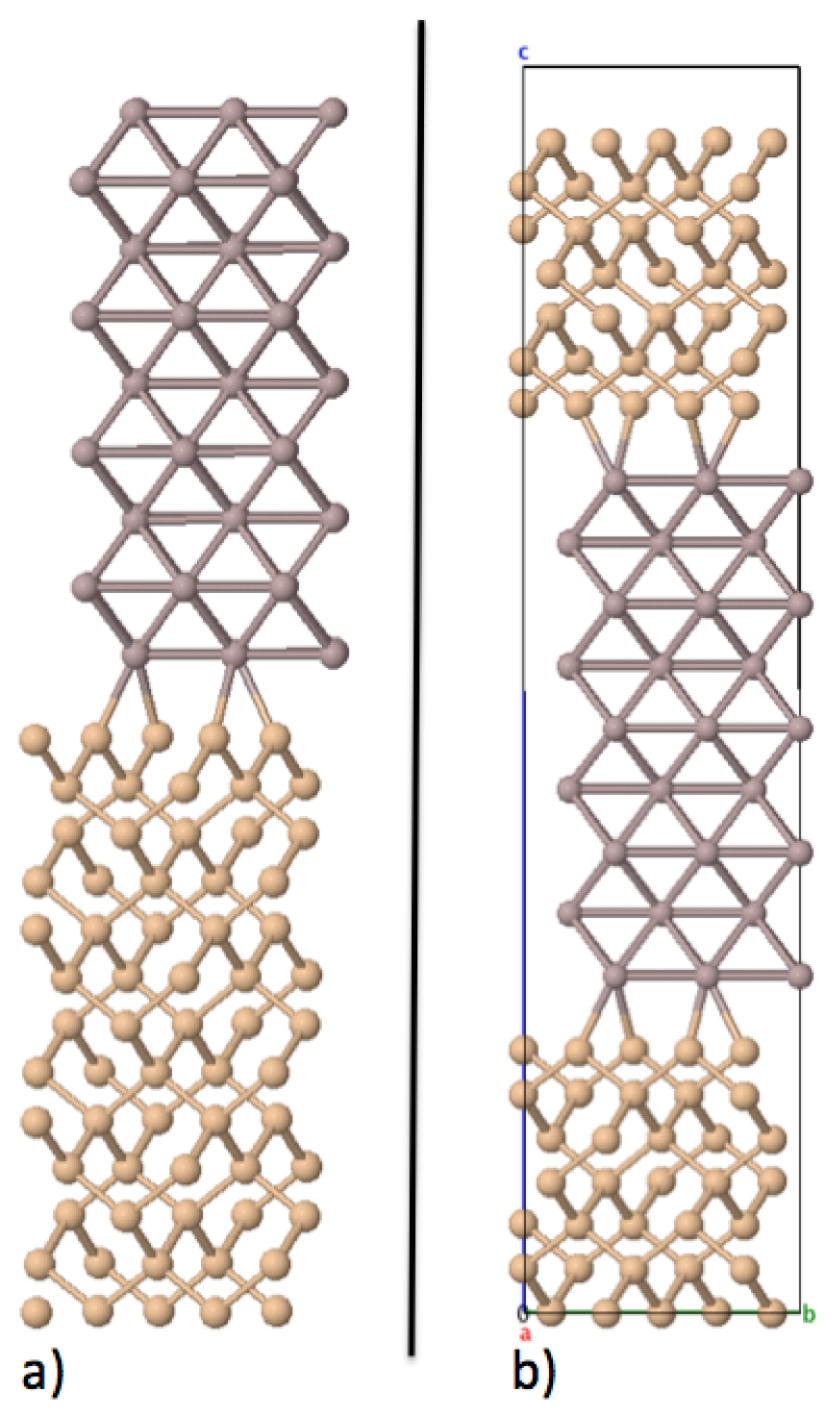
\includegraphics[scale=0.5]{structures}
\caption{Two possible interfaces consturced by Interface Builder: a) Deposit put
directly on the Substrate; b) Deposit "sandwiched" between two halves of
Substrate}
\label{Fig:struc}
\end{center}
\end{figure}


\section{Output}

The program outputs the following directories and files:
\begin{verbatim}
Deposit_hkl-Substrate_hkl
SCORE-hkl-hkl
\end{verbatim}
Additionally, the following files are crated:
\begin{verbatim}
summary.txt
summary.csv
FAILED_RESULTS.txt
\end{verbatim}

For each pair of Substrate - Deposit orientations a directory
\texttt{Deposit\_hkl-Substrate\_hkl} is created, where hkl denote Miller indices
for Deposit and Substrate respectively. The content of each of directory is
organized as follows: 

\begin{enumerate} 
\item The topmost subdirectory designates the alignment of Substrate and
Deposit and is numbered by integer from 0,...,m. The alignment 0 is always when
Deposit is put directly on Substrate, and alignment 1,2,3,...,m corresponds to the
situation when the Deposit it translated in the plane of the interface. The
number of alignments differs for each pair of Miller indices. 

\item In each directory corresponding the alignment, there is a set of new
directories named according to the pattern:
\texttt{Deposit\_hkl-Substrate\_hkl-N}, where \texttt{Deposit} and
\texttt{Substrate} are set to the names of the two materials, \texttt{hkl} are
Miller indices, and \texttt{N} is a number from \texttt{0,...,N} that labels the
configuration number. The configurations are created during lattice match and
with the increasing \texttt{N} the size of the interface also increases up
to the maximum given by \texttt{maxArea} in \texttt{options.dat} file.
Each such directory contains files with the following extensions:
\begin{itemize}
\item{\texttt{.xyz} - cartesian coordinates of interface}
\item{\texttt{.in}~  - coordinates in input file format for FHI-AIMS DFT code }
\item{\texttt{.gin}  - coordinates in input file format for Gulp MM code }
\item{\texttt{.idx} - miscellaneous information, such as number of atoms in
complex:substrate:deposit; indices of atom of the exposed surfaces; area of the
interface}
\end{itemize}
\end{enumerate}

Each directory \texttt{SCORE-hkl-hkl} contains the scoring information for the
given pair oh Substrate-Deposit orientations.

The file \texttt{summary.txt} contains big table that collects all the
parameters describing each created interface:
\begin{itemize}
\item length of the lattice vectors and interface area
\item stress in the interface, i.e. difference between lattice vectors of
Substrate and Deposit
\item Miller indices of Substrate and Deposit
\item distance between Substrate and Deposit
\item Score
\end{itemize}
File \texttt{summary.csv} contains the same information but in comma separated
format, that allows easy import to spreadsheet software such a Excel of
GoogleDocs.

The file \texttt{FAILED\_RESULTS.txt} lists the combinations of Substrate -
Deposit Miller indices for which surfaces with good lattice match couldn't be
find. 

\end{document}
